\newcommand{\linksize}{\scriptsize}

\begin{document}

\begin{frame}[plain]
  \titlepage
\end{frame}

\begin{frame}
  \frametitle{A Summer of Code}

  \begin{itemize}
    \item Google Summer of Code project, 2010
    \item Introduced initial JSON support in PostgreSQL
    \item authored by Joseph Adams
      \begin{itemize}
	\item Mentored by Andrew Dunstan 
    	\item Committed by Robert Haas
      \end{itemize}
    \item 
      {\linksize \href{https://git.postgresql.org/cgit/postgresql.git/commit/?id=5384a73f98d9829725186a7b65bf4f8adb3cfaf1}{Commit: Built-in JSON data type. \faExternalLink \\ (Tue Jan 31 11:48:23 2012 -0500)}}
    \begin{itemize} \item Appears in PostgreSQL 9.2 \item Released September 2012 \end{itemize}
	  \pause
    \item No internal structure
    \item No indexing
  \end{itemize}

\end{frame}
\note{ Worth pointing out?  Oracle 12c had JSON, released July 2013.  Microsoft SQL Server had JSON support in SQL Server 2016, released in June 2016. }

\begin{frame}[fragile]
  \frametitle{A Boost of Unstructure}
  \begin{itemize}
    \item Teodor Sigaev posts \textit{nested hstore} support \\
      \begin{itemize}
	\item[] \linksize \href{https://www.postgresql.org/message-id/flat/528274F3.3060403@sigaev.ru}{pgsql-hackers: nested hstore patch \faExternalLink
	\item[] (Tue, 12 Nov 2013 22:35:31 +0400)}
      \end{itemize}
    \item JSONB comes to life \\
      \begin{itemize}
	\item[] \linksize \href{https://git.postgresql.org/cgit/postgresql.git/commit/?id=d9134d0a355cfa447adc80db4505d5931084278a}{Commit: Introduce jsonb, a structured format for storing json. \faExternalLink
	\item[] (Sun Mar 23 16:40:19 2014 -0400)}
      \end{itemize}
      \pause
    \item Binary storage
    \item Allows indexing
  \end{itemize}

\end{frame}

\begin{frame}
  \frametitle{A Surprise of Easterners}
  \begin{itemize}
    \item February 2017: Oleg Bartunov posts about supporting the SQL standard syntax
      \begin{itemize}
	\item[] {\linksize \href{https://postgr.es/m/CAF4Au4w2x-5LTnN_bxky-mq4=WOqsGsxSpENCzHRAzSnEd8+WQ@mail.gmail.com}{pgsql-hackers: SQL/JSON in PostgreSQL \faExternalLink
	\item[] (Tue, 28 Feb 2017 22:08:43 +0300)}}
      \end{itemize}
    \item A 431 kB, 15000 lines patch!
    \item Authors: Nikita Glukhov, Teodor Sigaev, Oleg Bartunov, Alexander Korotkov
  \end{itemize}
\end{frame}

\begin{frame}
  \frametitle{A List of Functions}
  \centering 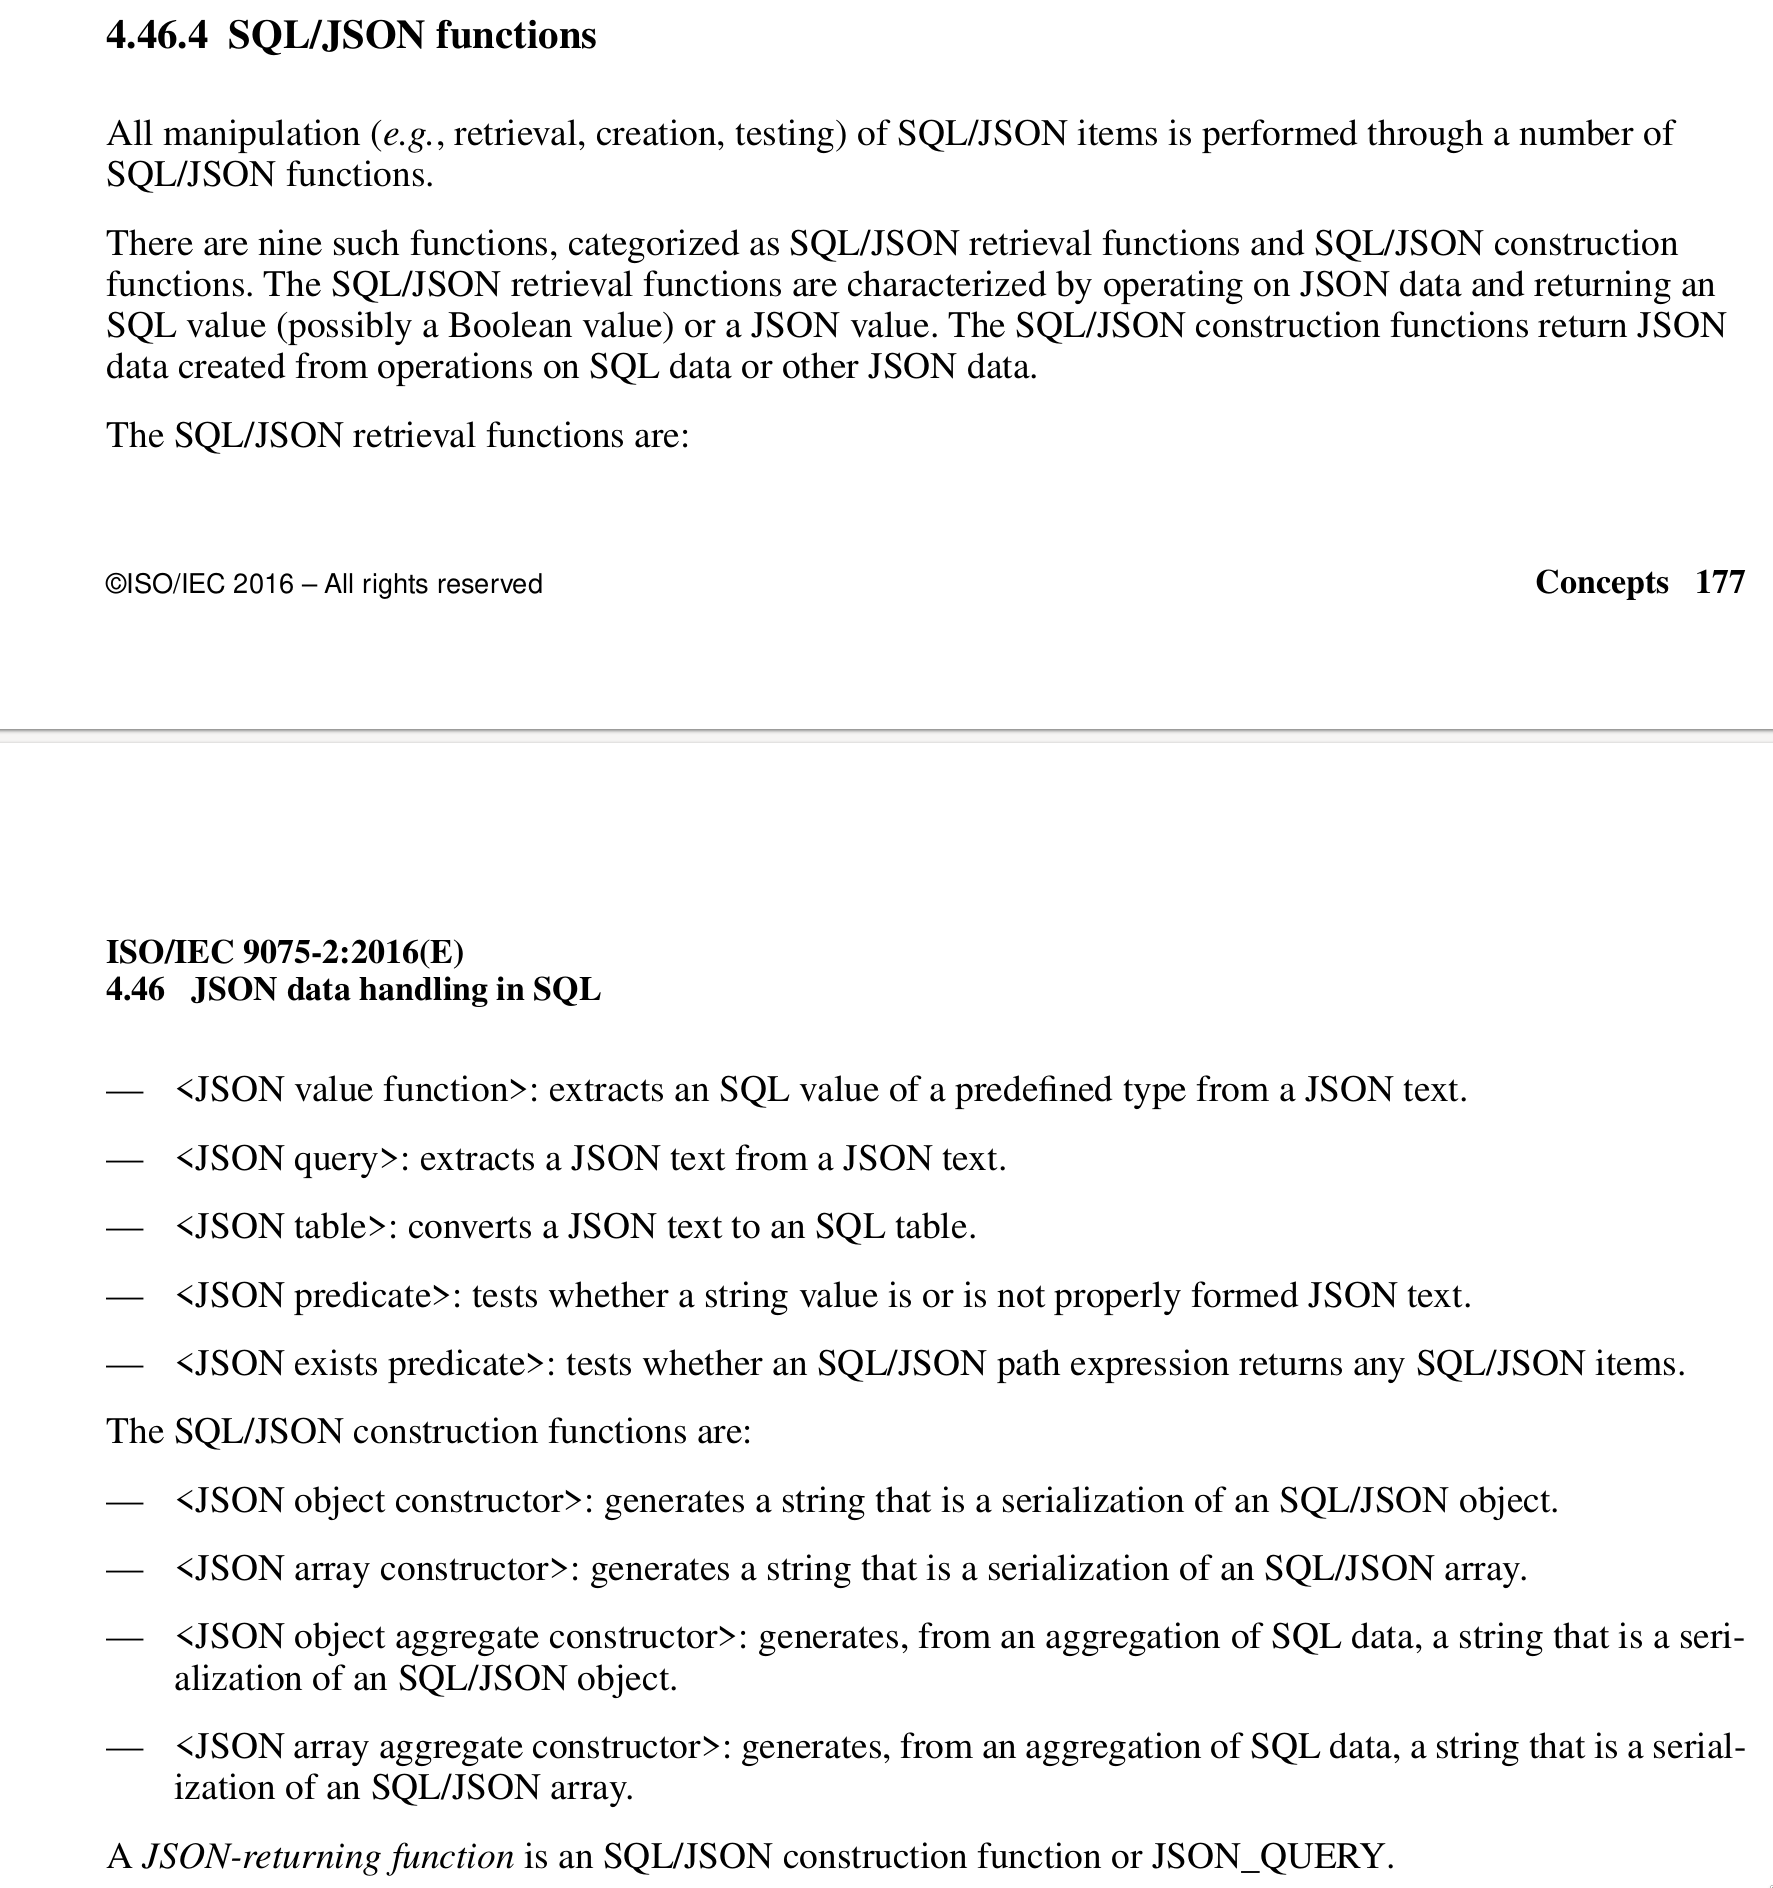
\includegraphics[height=0.9\textheight, frame]{sqljson_functions.png}
\end{frame}
\note{These are screenshots from the SQL 2016 standard, the first to include JSON support. It was released in November 2016, four months before Oleg posted their patch.}

\begin{frame}
  \frametitle{A List of Functions (1)}
  \centering 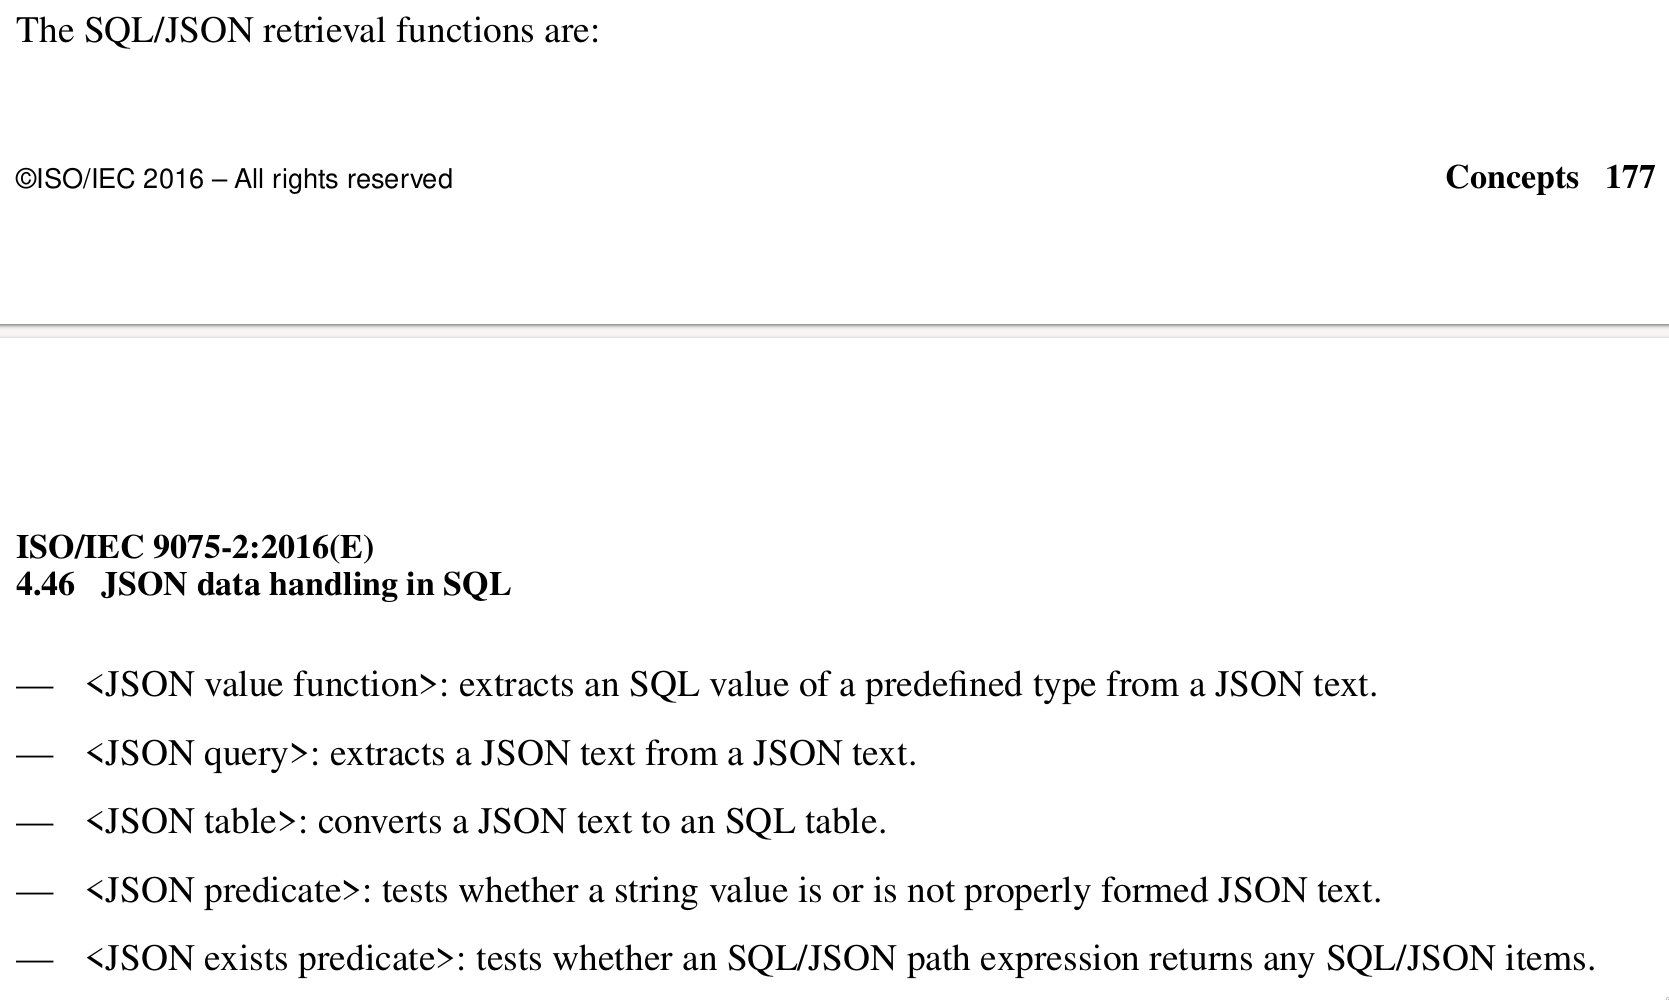
\includegraphics[width=\textwidth, frame]{sqljson_functions_1.png}
\end{frame}

\begin{frame}
  \frametitle{A Definition of Datatype}
  \centering 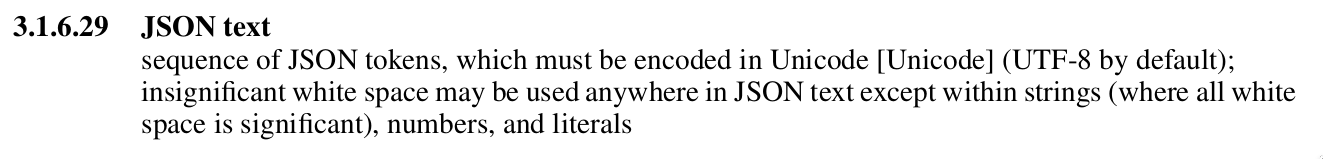
\includegraphics[width=\textwidth, frame]{jsontext.png}
\end{frame}

\begin{frame}
  \frametitle{A List of Functions (2)}
  \centering 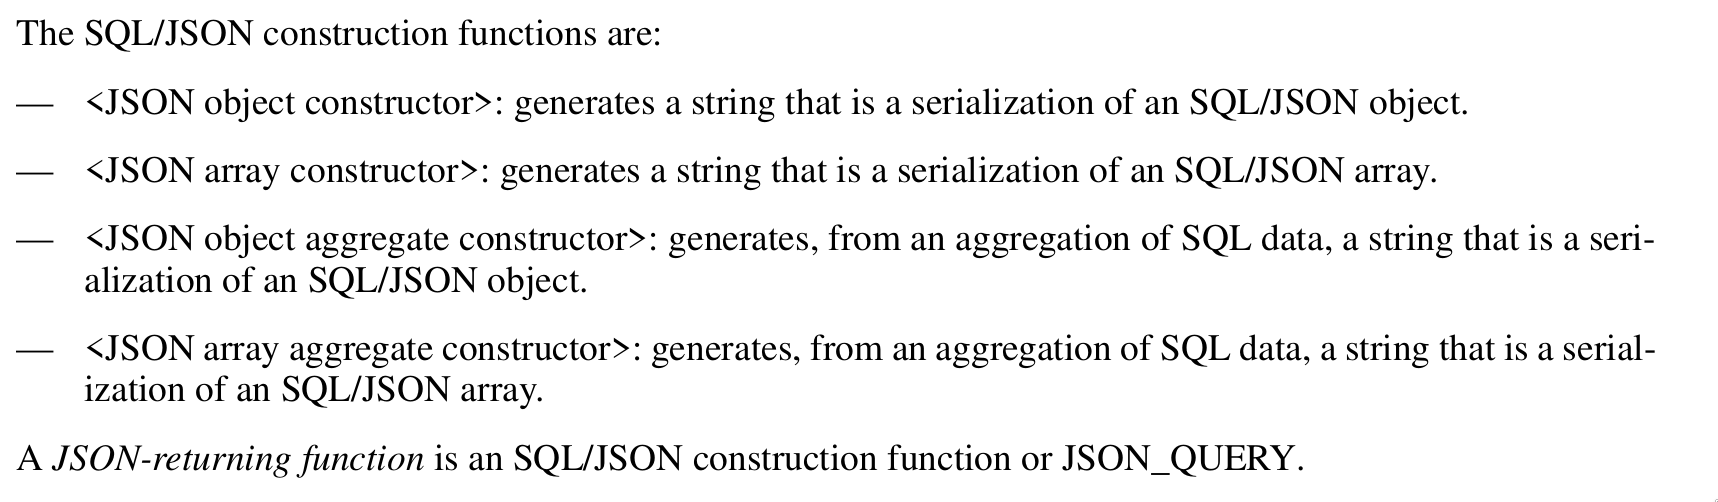
\includegraphics[width=\textwidth, frame]{sqljson_functions_2.png}
\end{frame}

\begin{frame}
  \frametitle{A Disaster of Commitments}

  \begin{itemize}
    \item First commit: March 22 2022, 17:32
    \item Immediately reverted at 19:56
      \pause
    \item Further 9 commits: from March 27th 2022 until April 7th
    \item Plus various later fixups
      \pause
    \item Everything (23 commits) reverted again in September 2022
      \pause
    \item Fundamental problem: catching parse errors
  \end{itemize}
\end{frame}

\begin{frame}
  \frametitle{A Capture of Errors}

  \begin{itemize}
    \item \textit{Soft errors} came about
    \item A new mechanism to capture errors before they're thrown
    \item More robust and performant
  \end{itemize}
  \centering \only<2>{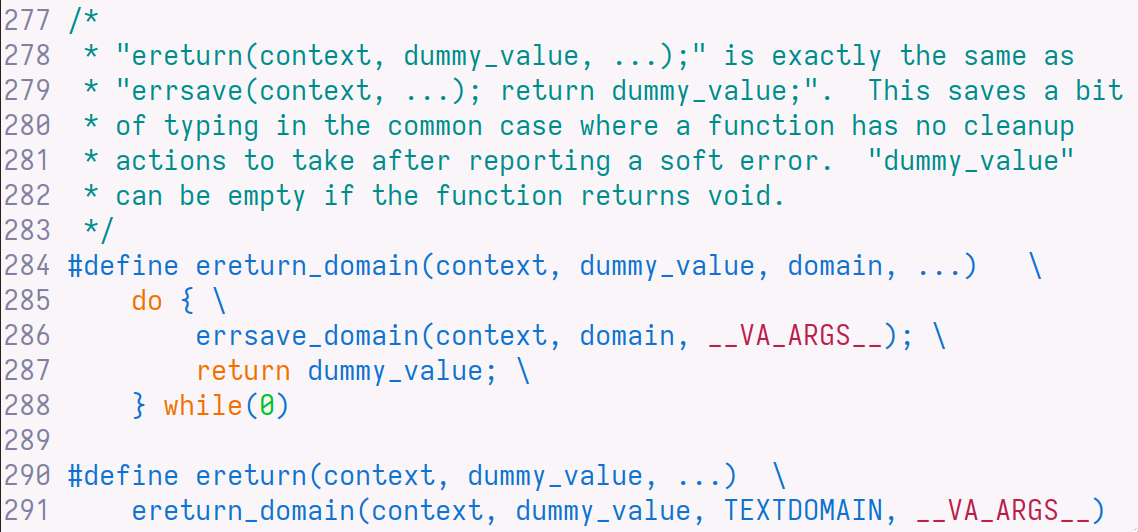
\includegraphics[width=\textwidth,frame]{ereturn.png}}
\end{frame}
\note{\texttt{ereturn()} and \texttt{errsave()} are Postgres C functions that improve on the model
implemented by \texttt{ereport()}.}

\begin{frame}[plain]
  \frametitle{A Capture of Errors (1)}
  \centering 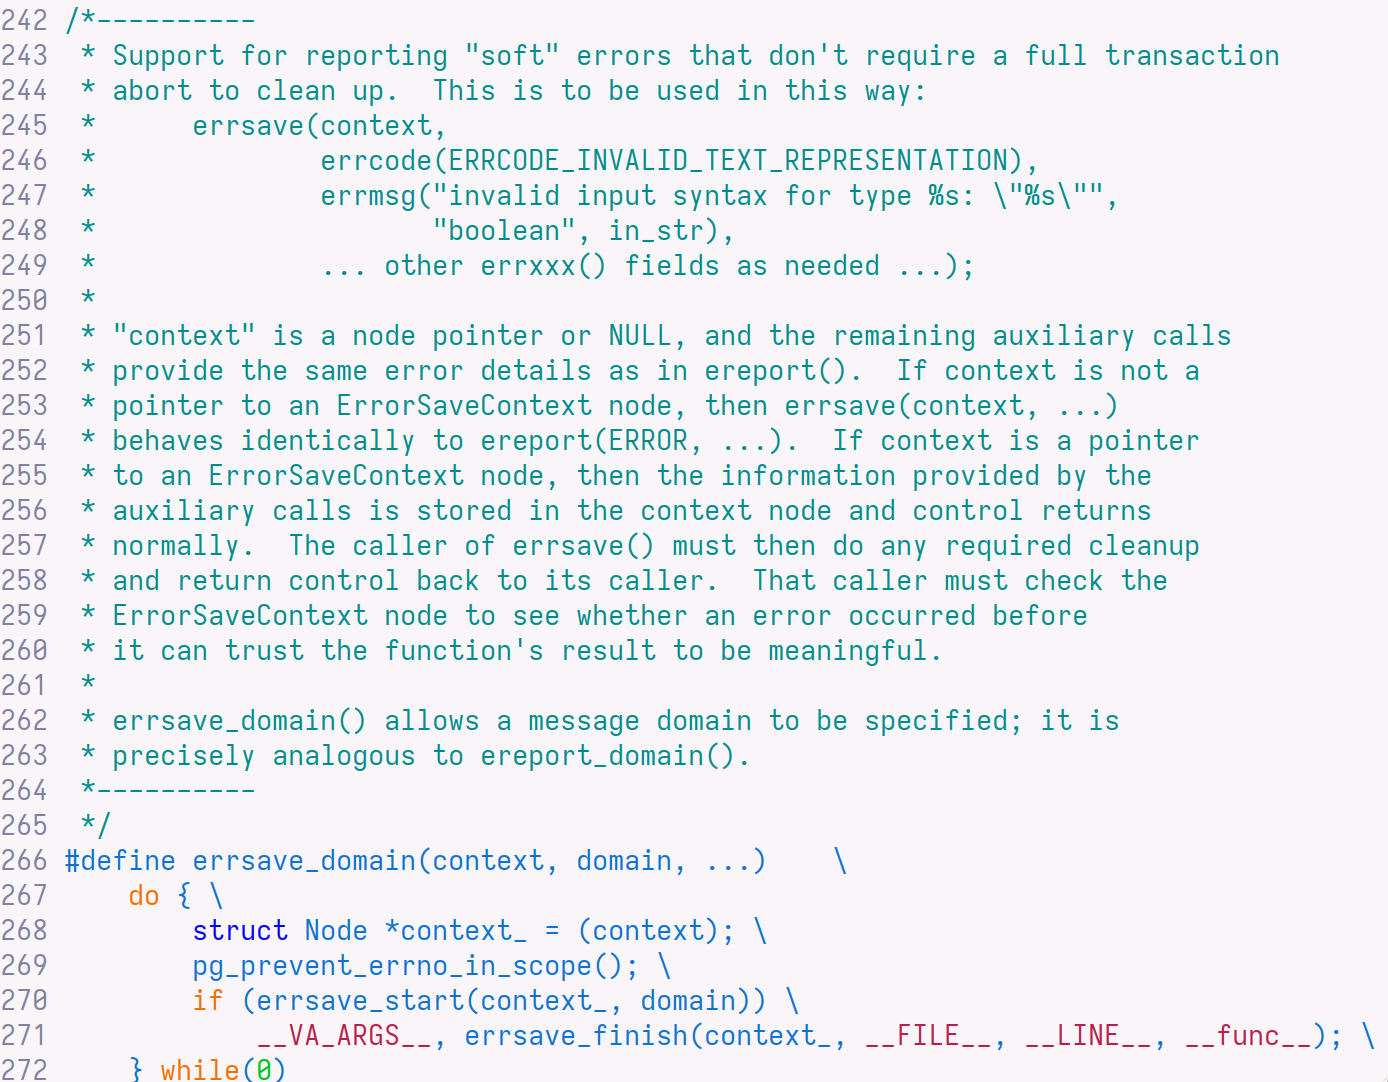
\includegraphics[height=0.9\textheight,frame]{errsave.png}
\end{frame}

\begin{frame}[plain]
  \frametitle{A Set of Updates}
  \begin{itemize}
    \item Amit Langote picks up the baton
      \begin{itemize}
\item[] \linksize \href{https://www.postgresql.org/message-id/flat/CA+HiwqHROpf9e644D8BRqYvaAPmgBZVup-xKMDPk-nd4EpgzHw@mail.gmail.com}{pgsql-hackers: SQL/JSON revisited \faExternalLink
	\item[] (Wed, 28 Dec 2022 16:28:29 +0900)}
      \end{itemize}
  \end{itemize}

  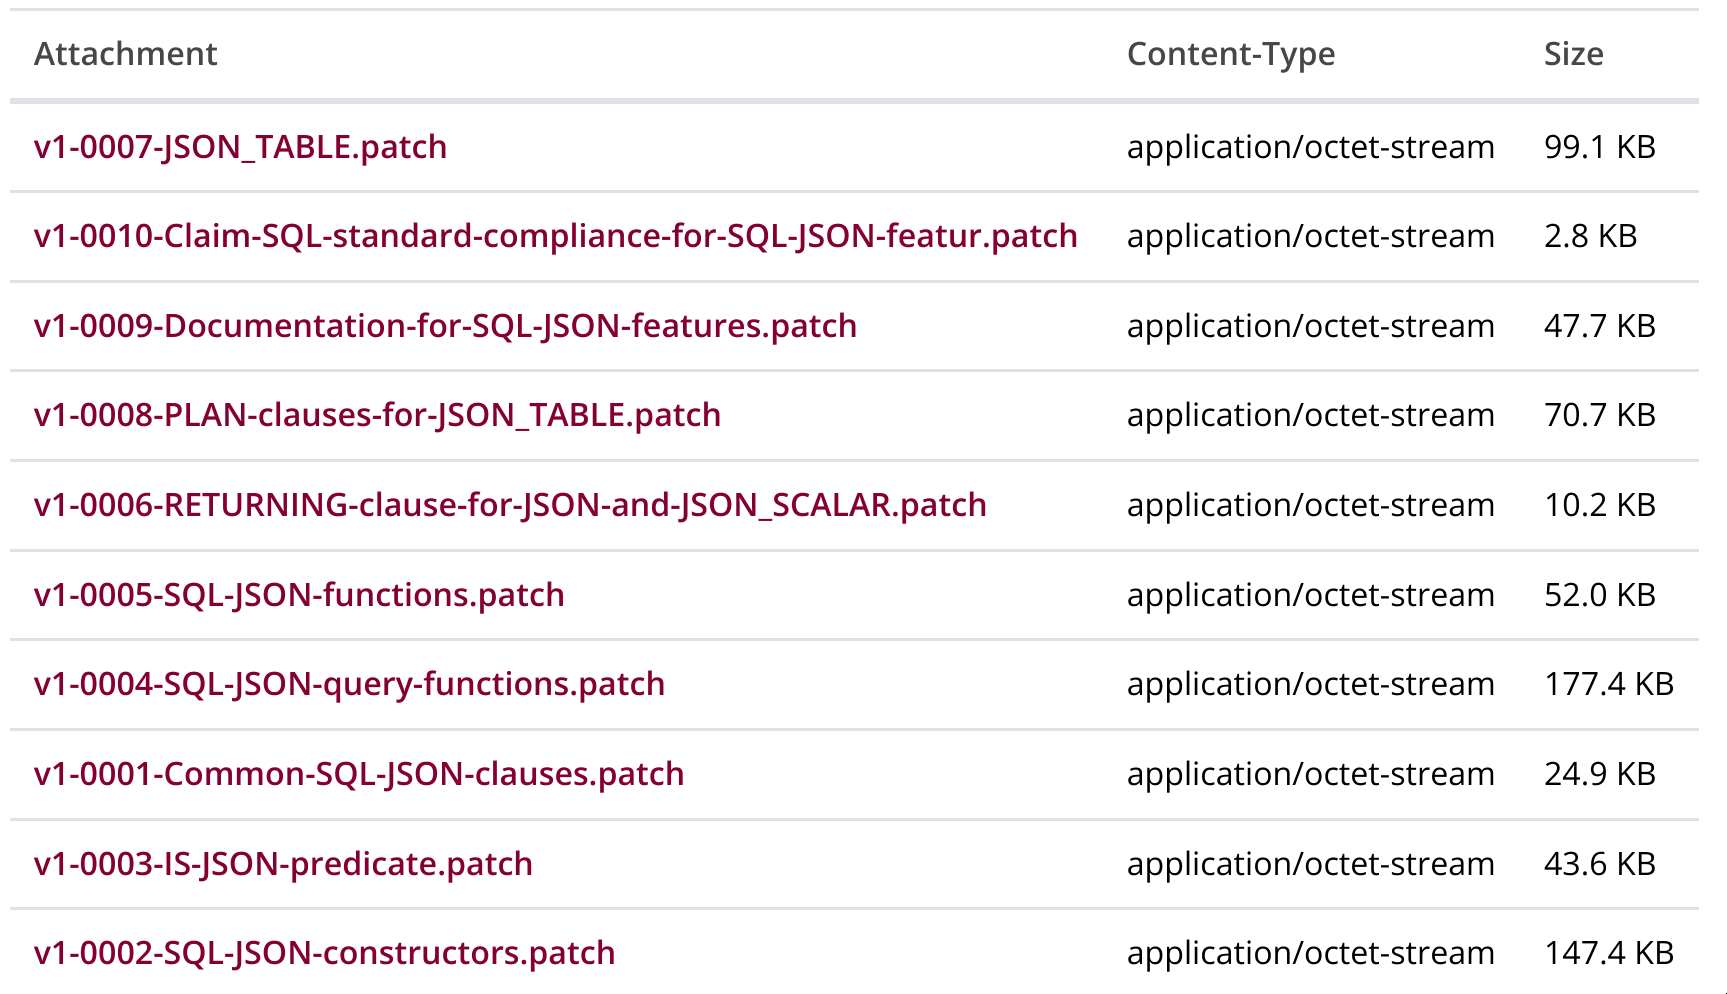
\includegraphics[width=\textwidth,frame]{patchlist-20221228.png}

\end{frame}

\begin{frame}
  \frametitle{A First of Many}
  \begin{itemize}
    \item Álvaro Herrera commits SQL/JSON constructors
    \item It finally sticks!
      \begin{itemize}
	\item[] \linksize \href{https://git.postgresql.org/cgit/postgresql.git/commit/?id=7081ac46ace8c459966174400b53418683c9fe5c}{Commit: SQL/JSON: add standard JSON constructor functions \faExternalLink
	\item[] (Wed Mar 29 12:11:36 2023 +0200)}
      \end{itemize}

    \item[]

    \item Squash of Amit's 0001, 0002, and parts of 0009
    \item[]

    \item \texttt{JSON\_ARRAY()}
    \item \texttt{JSON\_OBJECT()}
    \item \texttt{JSON\_ARRAYAGG()}
    \item \texttt{JSON\_OBJECTAGG}()
  \end{itemize}

\end{frame}

\begin{frame}[fragile]
  \frametitle{\texttt{JSON\_ARRAY()}}
  \begin{lstlisting}
JSON_ARRAY ( [ { value_expression [ FORMAT JSON ] } [, ...] ]
             [ { NULL | ABSENT } ON NULL ]
             [ RETURNING data_type [ FORMAT JSON [ ENCODING UTF8 ] ] ])

JSON_ARRAY ( [ query_expression ]
             [ RETURNING data_type [ FORMAT JSON [ ENCODING UTF8 ] ] ])
  \end{lstlisting}

    \begin{onlyenv}<2>
      \begin{lstlisting}
SELECT JSON_ARRAY(1+1, current_date,
                  '{"eek" : "ugly" }',
                  '{"happiness":"yes"}' FORMAT JSON);

                           json_array                            
─────────────────────────────────────────────────────────────────
 [2, "2024-05-26", "{\"eek\" : \"ugly\" }", {"happiness":"yes"}]
    \end{lstlisting}
    \end{onlyenv}
    \begin{onlyenv}<3>
      \begin{lstlisting}
SELECT JSON_ARRAY( SELECT relname FROM pg_class LIMIT 3 );

                         json_array                         
────────────────────────────────────────────────────────────
 ["postgres_log", "pg_toast_43619", "pg_toast_43619_index"]
    \end{lstlisting}
    \end{onlyenv}

    \begin{onlyenv}<4>
      \begin{lstlisting}
SELECT (JSON_ARRAY( '{"answer" : 42}' FORMAT JSON,
                    '{"question": "?"}' FORMAT JSON
        RETURNING JSONB))[0];

   json_array   
────────────────
 {"answer": 42}
      \end{lstlisting}
    \end{onlyenv}

    \begin{onlyenv}<5>
      \begin{lstlisting}
SELECT JSON_ARRAY( 1, NULL, 3 NULL ON NULL );

  json_array    
──────────────
 [1, null, 3]
      \end{lstlisting}
    \end{onlyenv}
\end{frame}
\note{The ``eek:ugly'' bit is just text, not a JSON object, which is why the quotes have been escaped by backslashes; by contrast, specifying \texttt{FORMAT JSON} lets the parser understand that the value given is a JSON element.

\texttt{RETURNING JSONB} makes it produce a JSONB object, which is why the array subscripting work. It doesn't with plain \texttt{JSON} datatype.
}

\begin{frame}[fragile]
  \frametitle{\texttt{JSON\_OBJECT()}}

  \begin{lstlisting}
JSON_OBJECT ( [ { key_expression { VALUE | ':' } value_expression
	        [ FORMAT JSON [ ENCODING UTF8 ] ] }[, ...] ]
	      [ { NULL | ABSENT } ON NULL ]
	      [ { WITH | WITHOUT } UNIQUE [ KEYS ] ]
	     [ RETURNING data_type [ FORMAT JSON [ ENCODING UTF8 ] ] ])
  \end{lstlisting}

  \begin{onlyenv}<2>
    \begin{lstlisting}
SELECT JSON_OBJECT('theKey' : 'theValue',
		   ('nother' || 'key') VALUE current_date,
		   'theKey' : null
		   ABSENT ON NULL);

                     json_object                     
─────────────────────────────────────────────────────
 {"theKey" : "theValue", "notherkey" : "2024-05-27"}
    \end{lstlisting}
  \end{onlyenv}

  \begin{onlyenv}<3>
    \begin{lstlisting}
SELECT JSON_OBJECT('theKey' : 'value 1',
		   'theKey' : 'value 2'
		   WITH UNIQUE KEYS);
ERROR:  duplicate JSON object key value: "theKey"
    \end{lstlisting}
  \end{onlyenv}

  \begin{onlyenv}<4>
  \begin{itemize} \item Alert of consistency loss \end{itemize}
    \begin{lstlisting}
SELECT JSON_OBJECT('the' || 'Key' : 'theValue',
                   ('the' || 'Key') VALUE current_date
                   WITHOUT UNIQUE KEYS
		   RETURNING jsonb);
       json_object        
──────────────────────────
 {"theKey": "2024-05-27"}
    \end{lstlisting}
  \end{onlyenv}

\end{frame}

\note{
When using \texttt{WITHOUT UNIQUE KEYS} (or omitting that clause), both values are present in the output; but jsonb ignores values other than the last for a given key, so these two things cause a value to be lost.
}

\begin{frame}[fragile]
  \frametitle{\texttt{JSON\_ARRAYAGG()}}
    \begin{lstlisting}
JSON_ARRAYAGG ( [ value_expression ] [ ORDER BY sort_expression ]
	        [ { NULL | ABSENT } ON NULL ]
	        [ RETURNING data_type
		         [ FORMAT JSON [ ENCODING UTF8 ] ] ])
    \end{lstlisting}

  \begin{onlyenv}<2>
    \begin{lstlisting}
SELECT last_name, JSON_ARRAYAGG(first_name ORDER BY first_name)
       FROM actor GROUP BY last_name LIMIT 3;

 last_name │           json_arrayagg            
───────────┼────────────────────────────────────
 AKROYD    │ ["CHRISTIAN", "DEBBIE", "KIRSTEN"]
 ALLEN     │ ["CUBA", "KIM", "MERYL"]
 ASTAIRE   │ ["ANGELINA"]
    \end{lstlisting}
  \end{onlyenv}
\end{frame}
\note{The data here comes from the \textit{pagila} sample database. It is more
heavily used later to produce a largish JSON array with some substructure.}

\begin{frame}[fragile]
  \frametitle{\texttt{JSON\_OBJECTAGG()}}

  \begin{onlyenv}<1>
\begin{lstlisting}
JSON_OBJECTAGG ( [ { key_expression { VALUE | ':' } value_expression } ]
                 [ { NULL | ABSENT } ON NULL ]
                 [ { WITH | WITHOUT } UNIQUE [ KEYS ] ]
             [ RETURNING data_type [ FORMAT JSON [ ENCODING UTF8 ] ] ])
\end{lstlisting}
  \end{onlyenv}

  \begin{onlyenv}<2>
    \begin{lstlisting}
SELECT a.address, jsonb_pretty(
    JSON_OBJECTAGG(staff_id : format('%s %s', first_name, last_name)
                   RETURNING jsonb))
    FROM staff JOIN store USING (store_id) JOIN address a
                 ON (store.address_id = a.address_id)
GROUP BY store_id, a.address_id LIMIT 1;

      address      │          jsonb_pretty          
───────────────────┼────────────────────────────────
 569 Baicheng Lane │ {                             ↵
                   │     "6": "Theo Harber",       ↵
                   │     "27": "Mercedes Gislason",↵
                   │     "36": "Flor Toy",         ↵
                   │     "1421": "Drew Fahey",     ↵
                   │     "1436": "Tyree Dicki",    ↵
                   │     "1471": "Dan Kling"       ↵
                   │ }
    \end{lstlisting}
  \end{onlyenv}
\end{frame}

\begin{frame}[fragile]
  \frametitle{A Last of Sixteen}
  \begin{itemize}
    \item Álvaro Herrera commits the \texttt{IS JSON} predicate
      \begin{itemize}
	\item[] \linksize \href{https://git.postgresql.org/cgit/postgresql.git/commit/?id=6ee30209a6f161d0a267a33f090c70c579c87c00}{Commit: SQL/JSON: support the IS JSON predicate \faExternalLink
	\item[] (Fri Mar 31 22:34:04 2023 +0200)}
      \end{itemize}
    \item[]
    \item \texttt{IS JSON [VALUE]}
    \item \texttt{IS JSON ARRAY}
    \item \texttt{IS JSON OBJECT}
    \item \texttt{IS JSON SCALAR}
\pause
    \item[]<2>
    \item<2> Nothing else would get done for 16, sadly
  \end{itemize}

  \begin{onlyenv}<3>
    \begin{lstlisting}
SELECT '{"xyzxz": 456}' IS JSON OBJECT;
 ?column? 
──────────
 t
    \end{lstlisting}
  \end{onlyenv}
\end{frame}

\begin{frame}
  \frametitle{A Completion of Efforts}

  \begin{itemize}
    \item Amit Langote runs the final marathon
      \begin{itemize}
	\item[] \linksize \href{https://www.postgresql.org/message-id/flat/CA+HiwqE4XTdfb1nW=Ojoy_tQSRhYt-q_kb6i5d4xcKyrLC1Nbg@mail.gmail.com}{pgsql-hackers: remaining sql/json patches \faExternalLink
	\item[] (Mon, 19 Jun 2023 17:31:57 +0900)}
      \end{itemize}
  \end{itemize}

  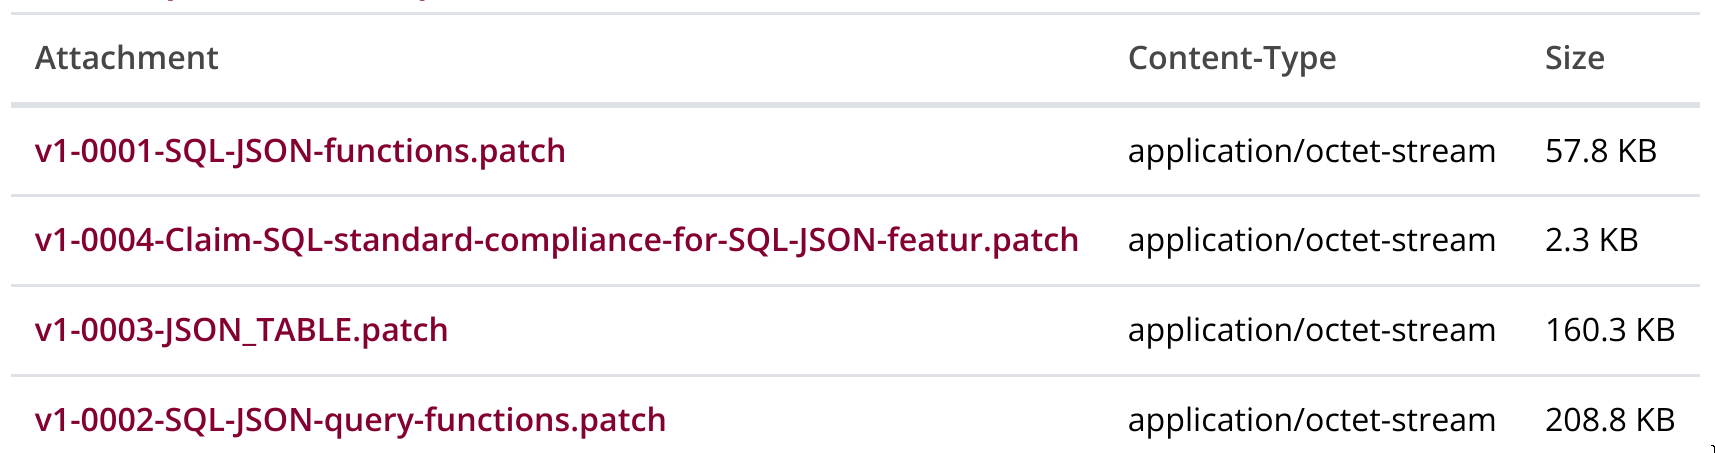
\includegraphics[width=\textwidth,frame]{patchlist-20230621.png}
\end{frame}

\begin{frame}
\frametitle{An Update of Standards}

\centering
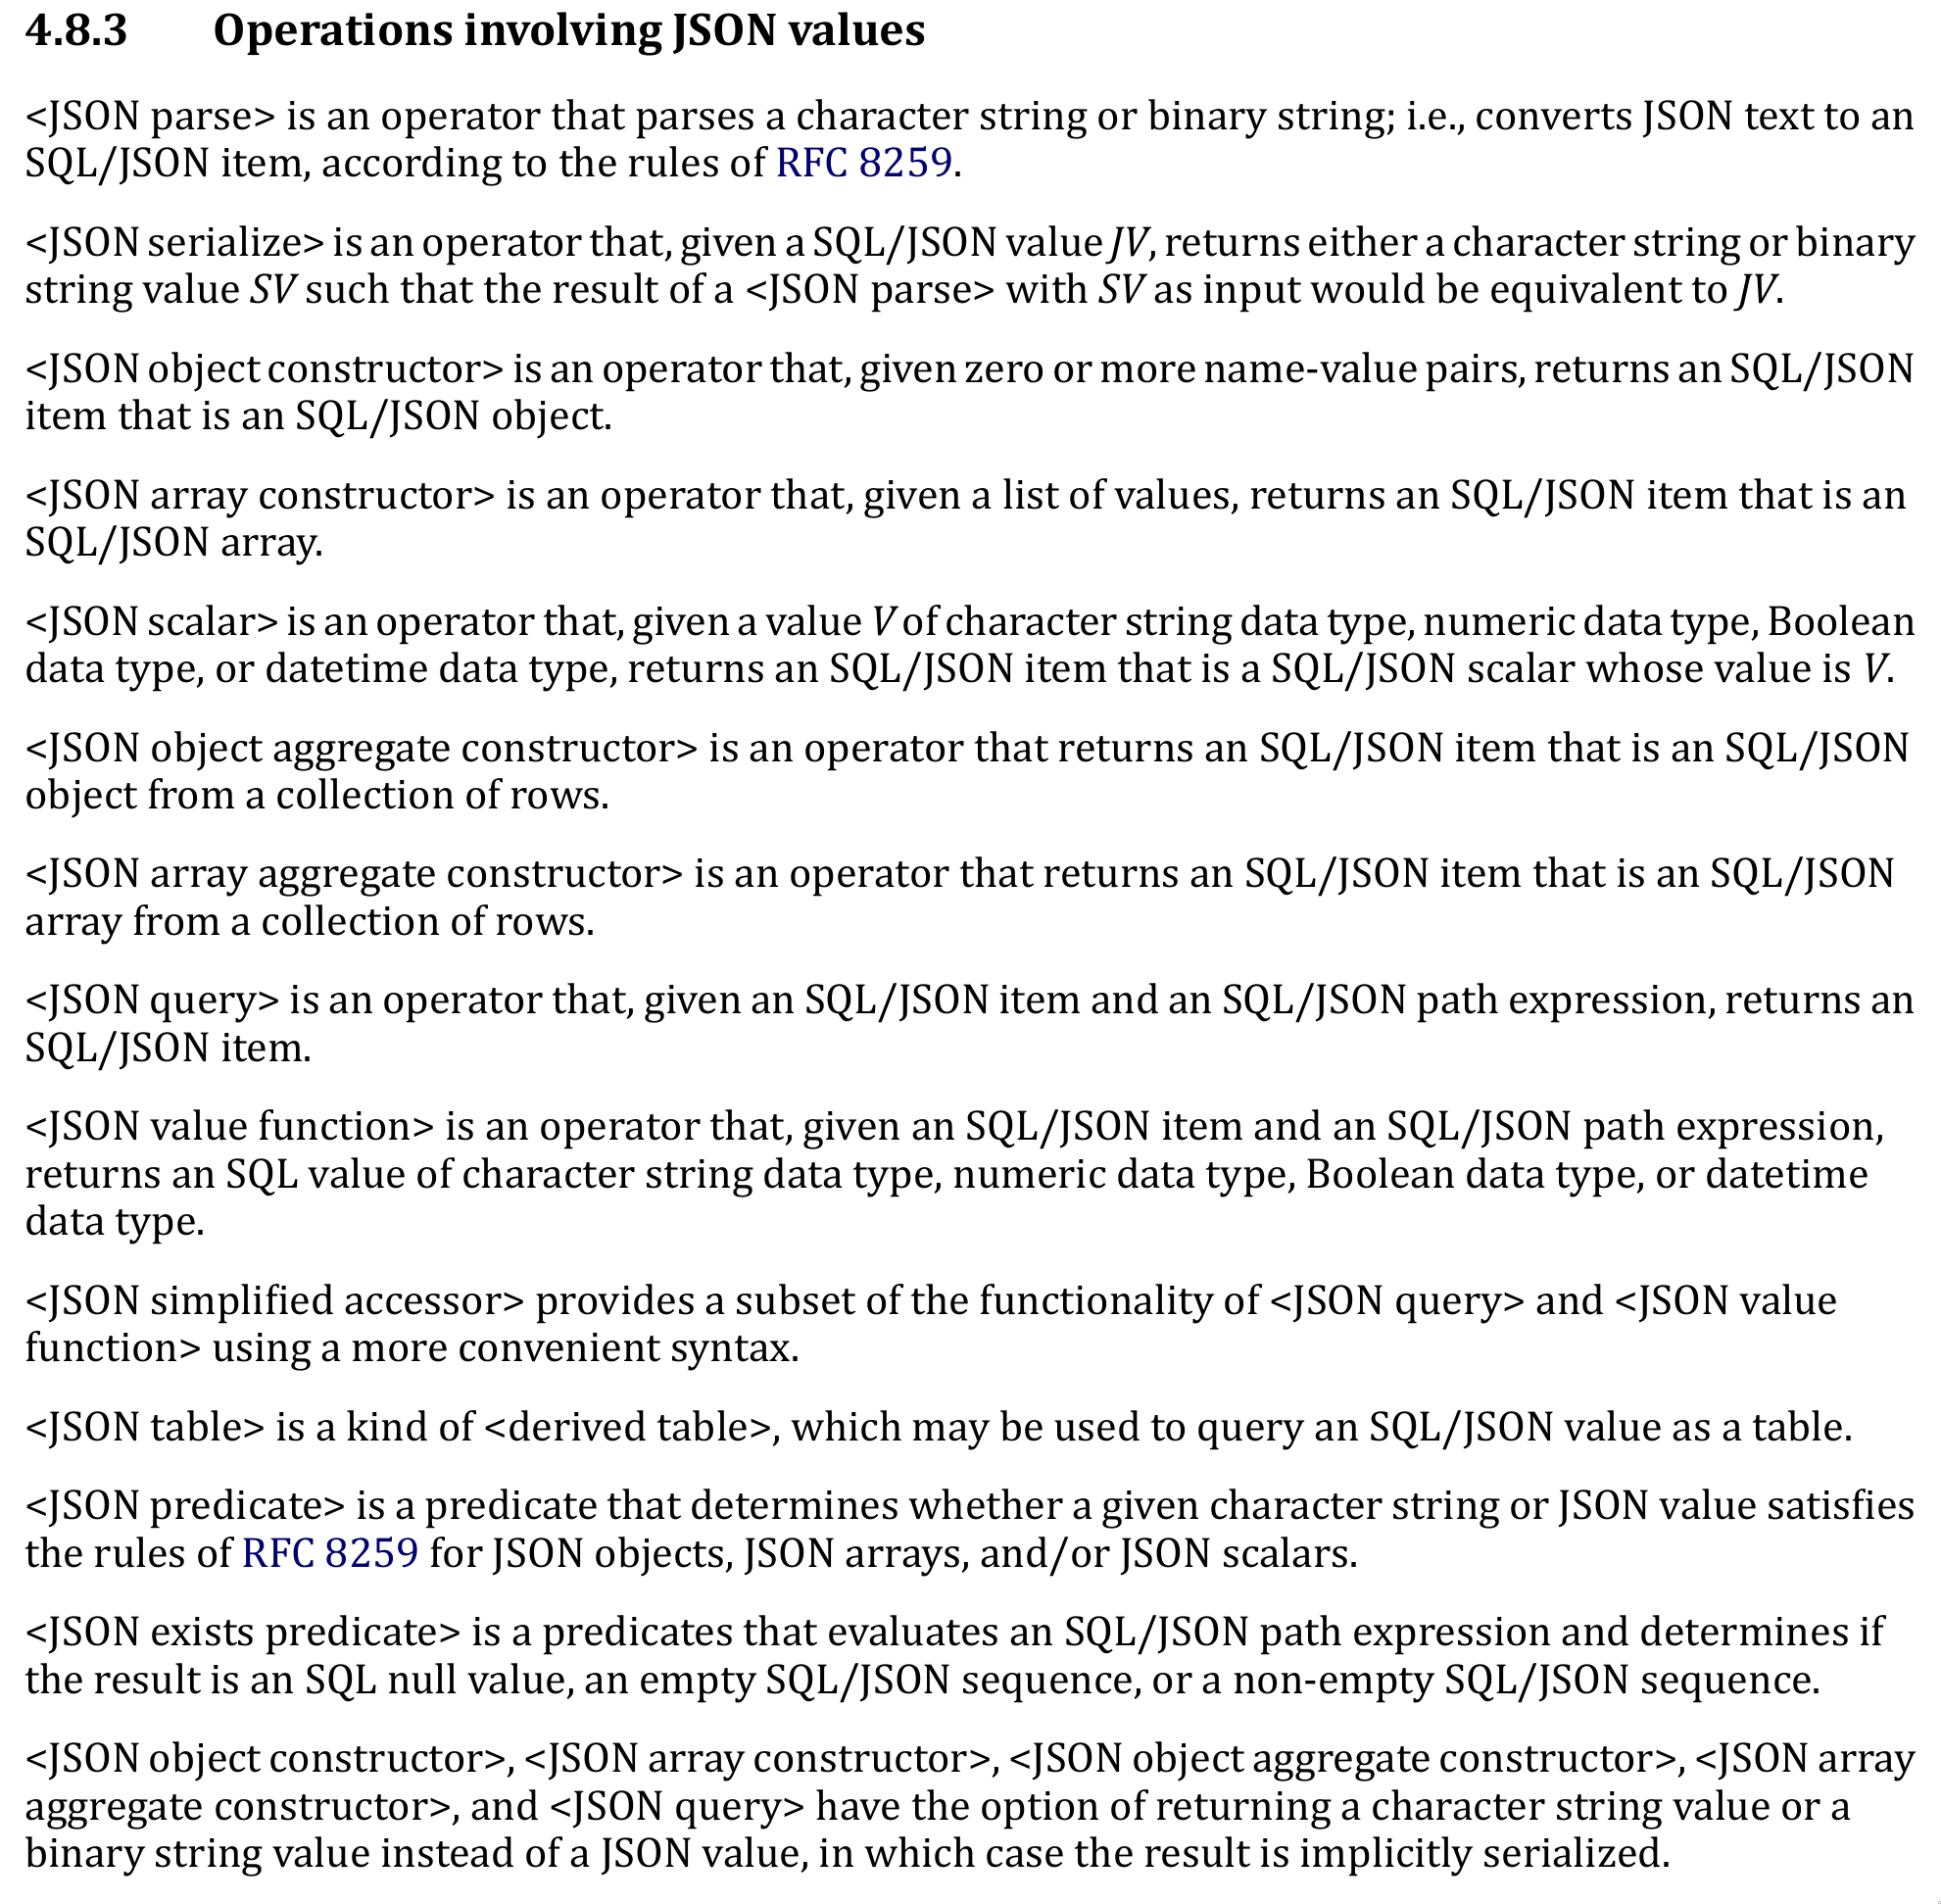
\includegraphics[height=0.9\textheight,frame]{sql2023.png}
\end{frame}

\begin{frame}[fragile]
  \frametitle{A Companionship of Constructors}

  \begin{itemize}
    \item Amit Langote commits more constructors
      \begin{itemize}
	\item[] \linksize \href{https://git.postgresql.org/cgit/postgresql.git/commit/?id=03734a7fed7d924679770adb78a7db8a37d14188}{Commit: Add more SQL/JSON constructor functions \faExternalLink
	\item[] (Wed Jul 26 17:08:33 2023 +0900)}
      \end{itemize}

    \item \texttt{JSON()}
    \item \texttt{JSON\_SCALAR()}
    \item \texttt{JSON\_SERIALIZE()}
  \end{itemize}

  \begin{onlyenv}<2>
    \begin{lstlisting}
JSON ( expression [ FORMAT JSON [ ENCODING UTF8 ]]
       [ { WITH | WITHOUT } UNIQUE [ KEYS ]] )
    
SELECT JSON('{"hike": [1, 2, {"answer":42, "question":null}]}');

                       json                       
──────────────────────────────────────────────────
 {"hike": [1, 2, {"answer":42, "question":null}]}
    \end{lstlisting}
  \end{onlyenv}

  \begin{onlyenv}<3>
    \begin{lstlisting}
JSON_SCALAR ( expression )

SELECT JSON_SCALAR('xyzxz');
 json_scalar 
─────────────
 "xyzxz"
    \end{lstlisting}
  \end{onlyenv}

  \begin{onlyenv}<4>
    \begin{lstlisting}
JSON_SERIALIZE ( expression [ FORMAT JSON [ ENCODING UTF8 ] ]
                 [ RETURNING data_type
		        [ FORMAT JSON [ ENCODING UTF8 ] ] ] )
			
SELECT pg_typeof(JSON_SERIALIZE('{"whatever": "some values"}'
                 RETURNING text));
 pg_typeof 
───────────
 text
    \end{lstlisting}
  \end{onlyenv}
\end{frame} 

\begin{frame}
  \frametitle{A Definition of Paths}
  \begin{itemize}
    \item Amit Langote commits SQL/JSON query functions
      \begin{itemize}
	\item[] \linksize \href{https://git.postgresql.org/cgit/postgresql.git/commit/?id=6185c9737cf48c9540782d88f12bd2912d6ca1cc}{Commit: Add SQL/JSON query functions \faExternalLink
	\item[] (Thu Mar 21 17:07:03 2024 +0900)}
      \end{itemize}
    \item[]

    \item \texttt{JSON\_QUERY()}
    \item \texttt{JSON\_EXISTS()}
    \item \texttt{JSON\_VALUE()}
  \end{itemize}
\end{frame}

\begin{frame}[fragile]

\begin{itemize} \scriptsize \item (Data from \textit{pagila} sample database) \end{itemize}

\scriptsize
  \begin{lstlisting}[basicstyle=\tiny\ttfamily]
create table allstores as
with store_staff as (
select
   store_id,
   json_arrayagg(
         json_object('id' : staff.staff_id,
                   'name' : staff.first_name || ' ' ||
                            staff.last_name,
                'address' : json_object(
                            'street' : sa.address,
                          'district' : sa.district,
                               'zip' : sa.postal_code
			               )
                    )
                ) as staff
  from staff join store using (store_id)
             join address sa on (staff.address_id = sa.address_id)
  group by store_id)
  select json_arrayagg(json_object( 
           'id' : store.store_id,
      'manager' : mgr.first_name || ' ' || mgr.last_name,
        'staff' : store_staff.staff
      'address' : json_object('street': stoaddr.address,
                            'district': stoaddr.district,
                                 'zip': stoaddr.postal_code),
                   returning jsonb)
                      ) as alldata
from store
  join staff mgr on (store.manager_staff_id = mgr.staff_id)
  join store_staff on (store.store_id = store_staff.store_id)
  join address stoaddr on (store.address_id = stoaddr.address_id);
  \end{lstlisting}
\end{frame}

\begin{frame}
  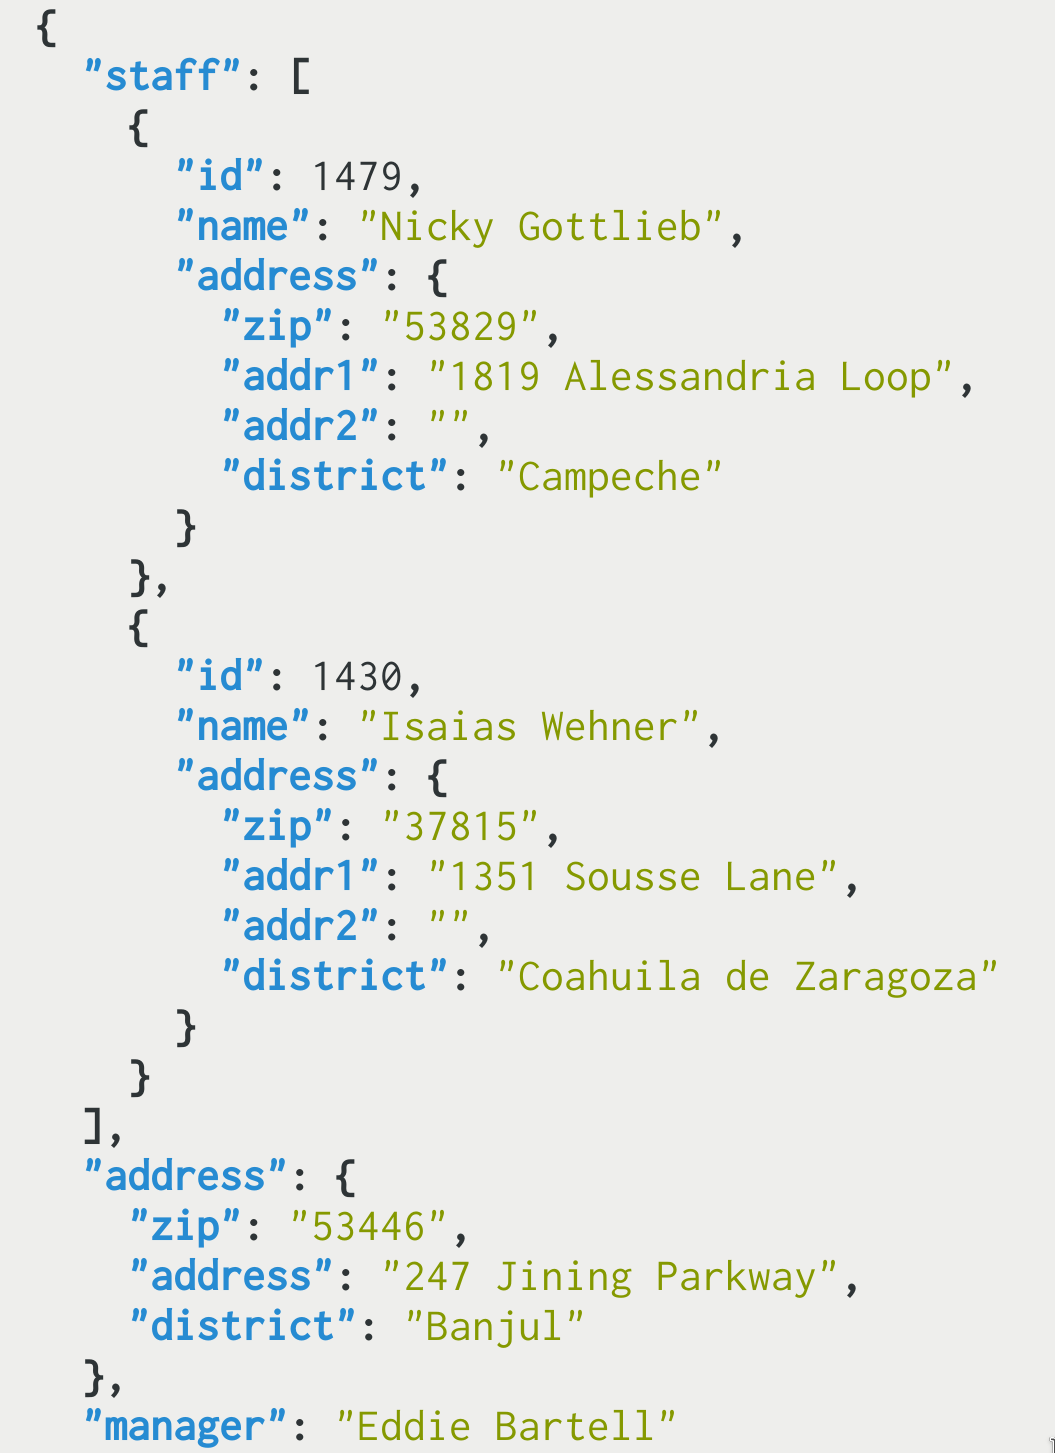
\includegraphics[height=0.9\textheight,frame]{sampledata.png}
\end{frame}

\begin{frame}[fragile]
  \frametitle{\texttt{JSON\_QUERY()}}

  \begin{lstlisting}
JSON_QUERY ( context_item,
       path_expression [ PASSING { value AS varname } [, ...]]
	    [ RETURNING data_type [ FORMAT JSON [ ENCODING UTF8 ] ] ]
     [ { WITHOUT | WITH [ CONDITIONAL | UNCONDITIONAL ] }
                                          [ ARRAY ] WRAPPER ]
     [ { KEEP | OMIT } QUOTES [ ON SCALAR STRING ] ]
     [ { ERROR | NULL | EMPTY [ ARRAY | OBJECT ] |
                                  DEFAULT expression } ON EMPTY ]
     [ { ERROR | NULL | EMPTY [ ARRAY | OBJECT ] |
                                  DEFAULT expression } ON ERROR ])
  \end{lstlisting}

  \begin{onlyenv}<2>
    \begin{lstlisting}
SELECT json_query(alldata,
            '$[$storeidx].manager' PASSING 42 AS storeidx
                  RETURNING JSON)    FROM allstores;

	 json_query   
      ────────────────
       "Kristel Bins"
    \end{lstlisting}
  \end{onlyenv}

\end{frame}

\begin{frame}[fragile]
  \frametitle{\texttt{JSON\_QUERY()}}
    \begin{lstlisting}
select jsonb_pretty(json_query(alldata, '$[2 to 4].staff[*].name'
            returning jsonb with wrapper))
    from allstores;

     jsonb_pretty      
───────────────────────
 [                    ↵
     "Mira Reynolds", ↵
     "Lexie Von",     ↵
     "Jeanene Rippin",↵
     "Jeannie Cronin",↵
     "Moon Ondricka", ↵
     "Juliette Kulas",↵
     "Thersa Daniel", ↵
     "Dee Zboncak"    ↵
 ]
    \end{lstlisting}
\end{frame}
%stopzone	Fixes Vim

\begin{frame}
  \frametitle{A Language of Inspection}

\begin{itemize}
  \item \href{https://www.postgresql.org/docs/17/functions-json.html\#FUNCTIONS-SQLJSON-PATH}{\texttt{jsonpath} documentation \faExternalLink}
      \begin{itemize}
	\item Authored by Nikita Glukhov and Teodor Sigaev
	\item Committed by Alexander Korotkov in PostgreSQL 12
	\item[] \linksize \href{https://git.postgresql.org/cgit/postgresql.git/commit/?id=72b6460336e86ad5cafd3426af6013c7d8457367}{Commit: Partial implementation of SQL/JSON path language \faExternalLink
	\item[] (Sat Mar 16 12:16:48 2019 +0300)}
      \end{itemize}
    \item[]
\end{itemize}

  \begin{description}
    \item[\texttt{\$}] The ``context item''
    \item[\texttt{\$var}] A variable in the PASSING clause
    \item[\texttt{.key}] Object member accessor
    \item[\texttt{.*}] Accessor for all direct members of object
    \item[\texttt{[index]}] Array member accessor
  \end{description}
\end{frame}

\begin{frame}
  \frametitle{A Language of Inspection (2)}
  \begin{description}
    \item[\texttt{[*]}] Accessor for all array members
    \item[\texttt{[index1, index2, ...]}] Scattered member accesor
    \item[\texttt{[start\_index to end\_index]}] Multi-item array member accessor
    \item[]
    \item[\texttt{.**}] Recursive accessor for object
    \item[\texttt{.**\{level\}}] Recursive accessor for object at specific level
    \item[\texttt{.**\{start\_level to end\_level\}}] Recursive, given levels
      \pause
    \item[]
    \item[\texttt{.\textit{function}()}] Function invocation
    \item[]
    \item modes \textit{lax} and \textit{strict}
  \end{description}
\end{frame}

\begin{frame}[fragile]
  \frametitle{A Filtering of Results}
  \begin{lstlisting}
SELECT jsonb_pretty(json_query(alldata,
       '$ ? (@.staff[*].address.district == "Santiago")' 
    RETURNING JSONB WITH ARRAY WRAPPER))
    FROM allstores;

                    jsonb_pretty                     
─────────────────────────────────────────────────────
 [                                                  ↵
     {                                              ↵
         "id": 243,                                 ↵
         "staff": [                                 ↵
             {                                      ↵
                 "id": 646,                         ↵
                 "name": "Joanie Schroeder",        ↵
                 "address": {                       ↵
                     "zip": "69517",                ↵
                     "street": "532 Toulon Street", ↵
                     "district": "Santiago"         ↵
                 }                                  ↵
             },                                     ↵
             {                                      ↵
                 "id": 702,                         ↵
    ...
  \end{lstlisting}
\end{frame}
%stopzone
%stopzone
%stopzone  % Three of these are needed to fix Vim here

\begin{frame}[fragile]
  \frametitle{An Insistence of Filters}

  \begin{lstlisting}
SELECT json_query(alldata,
'strict $[*] ? (@.staff[*].address.district == $loc).staff.size()'
  PASSING 'Santiago' AS loc ERROR ON ERROR)
FROM allstores;

 json_query 
────────────
 5 %*\pause*)

SELECT json_query(alldata,
  '$ ? (@.staff.size() > 7)
       ? (@.address.zip like_regex "^55").manager'
  RETURNING TEXT OMIT QUOTES) FROM allstores;

   json_query   
────────────────
 Danial Quitzon
  \end{lstlisting}  
%stopzone  % Fix Vim
\end{frame}
\note{The PASSING clause is used to give values that can be used in the jsonpath.
The value can come from the current data row.

A jsonpath can have multiple \texttt{?} symbols, which form a chain.
}

\begin{frame}[fragile]
  \frametitle{\texttt{JSON\_VALUE()}}

  \begin{lstlisting}
  JSON_VALUE ( context_item,
         path_expression [ PASSING { value AS varname } [, ...]]
	 [ RETURNING data_type ]
	 [ { ERROR | NULL | DEFAULT expression } ON EMPTY ]
	 [ { ERROR | NULL | DEFAULT expression } ON ERROR ]) %*\pause*)

SELECT JSON_VALUE(alldata,
'strict $[*] ? (@.staff[*].address.district == $loc).staff[1].name'
  PASSING 'Santiago' AS loc ERROR ON ERROR)
FROM allstores;

 json_value 
────────────
 Love Feest
  \end{lstlisting}
\end{frame}

\begin{frame}[fragile]
  \frametitle{\texttt{JSON\_EXISTS()}}

  \begin{lstlisting}
JSON_EXISTS ( context_item,
              path_expression [ PASSING { value AS varname } [, ...]]
              [ { TRUE | FALSE | UNKNOWN | ERROR } ON ERROR ])

  \end{lstlisting}

  \begin{itemize}
    \item Returns (Boolean) whether an item matches the search expression
    \item \texttt{ERROR ON ERROR} recommended
  \end{itemize}
\end{frame}

\begin{frame}
  \frametitle{A full-circle of Models}
  \begin{itemize}
    \item Amit Langote commits JSON\_TABLE

      \begin{itemize}
	\item[] \linksize \href{https://git.postgresql.org/cgit/postgresql.git/commit/?id=de3600452b61d1bc3967e9e37e86db8956c8f577}{Commit: Add basic JSON\_TABLE() functionality \faExternalLink
	\item[] (Thu Apr 4 20:20:15 2024 +0900)}
      \end{itemize}
    \item[]

    \item Amit Langote adds NESTED clause to JSON\_TABLE

      \begin{itemize}
	\item[] \linksize \href{https://git.postgresql.org/cgit/postgresql.git/commit/?id=bb766cde63b4f624d029b34c9cdd3d0a94fd5b46}{Commit: JSON\_TABLE: Add support for NESTED paths and columns \faExternalLink
	\item[] (Mon Apr 8 16:14:13 2024 +0900)}
      \end{itemize}
  \end{itemize}
\end{frame}
\note{I've called this a "full-circle" because JSON\_TABLE puts your data back in relational format,
while the previous functions consumed the tabular-formatted data to build JSON.}

\begin{frame}[fragile]
  \frametitle{\texttt{JSON\_TABLE()}}
  \begin{lstlisting}[basicstyle=\scriptsize\ttfamily]
JSON_TABLE (
    context_item, path_expression [ AS json_path_name ]
    [ PASSING { value AS varname } [, ...] ]
    COLUMNS ( json_table_column [, ...] )
    [ { ERROR | EMPTY } ON ERROR ]
)
                        where json_table_column is:
name FOR ORDINALITY
| name type
      [ FORMAT JSON [ENCODING UTF8]]
      [ PATH path_expression ]
      [ { WITHOUT | WITH } [ CONDITIONAL | UNCONDITIONAL ] [ARRAY] WRAPPER ]
      [ { KEEP | OMIT } QUOTES [ ON SCALAR STRING ] ]
      [ { ERROR | NULL | EMPTY { ARRAY | OBJECT } | DEFAULT expression }
                                                              ON EMPTY ]
      [ { ERROR | NULL | EMPTY { ARRAY | OBJECT } | DEFAULT expression }
                                                              ON ERROR ]
| name type EXISTS [ PATH path_expression ]
      [ { ERROR | TRUE | FALSE | UNKNOWN } ON ERROR ]
| NESTED [ PATH ] path_expression [ AS json_path_name ]
                  COLUMNS ( json_table_column [, ...] )
  \end{lstlisting}

\end{frame}

\begin{frame}[fragile]
  \frametitle{\texttt{JSON\_TABLE()}}
  \begin{lstlisting}
SELECT j.store_id, j.manager, jsonb_pretty(address)
  FROM allstores,
         json_table(alldata,
                '$[$storeid]' PASSING 42 AS storeidx
                COLUMNS (
                      store_id  integer path  '($.id)',
                      manager   text path '($.manager)',
                      address   jsonb path '($.address)'
                )
        ) j; %*\pause*)

 store_id │   manager    │             jsonb_pretty             
──────────┼──────────────┼──────────────────────────────────────
       46 │ Kristel Bins │ {                                   ↵
          │              │     "zip": "94352",                 ↵
          │              │     "street": "1213 Ranchi Parkway",↵
          │              │     "district": "Karnataka"         ↵
          │              │ }
  \end{lstlisting}
%stopzone
\end{frame}

\begin{frame}[fragile]
  \frametitle{\texttt{JSON\_TABLE()}}
  \begin{lstlisting}[basicstyle=\tiny\ttfamily]
SELECT j.* 
  FROM allstores,
         json_table(alldata,
                'strict $[*] ? (@.id == $storeid)' PASSING 42 AS storeidx
                COLUMNS (
                      store_id  integer path  '($.id)',
                      manager   text path '($.manager)', 
                      NESTED '$.staff[*]' columns
                        (name text path '$.name',
                         straddress text path '$.address.street'
                ))
        ) j;

─[ RECORD 1 ]──────────────────────
store_id   │ 42
manager    │ Lincoln Wisoky
name       │ Norris Wilderman
straddress │ 1135 Izumisano Parkway
─[ RECORD 2 ]──────────────────────
store_id   │ 42
manager    │ Lincoln Wisoky
name       │ Lester Stehr
straddress │ 698 Otsu Street
─[ RECORD 3 ]──────────────────────
store_id   │ 42
manager    │ Lincoln Wisoky
name       │ Brendon Thiel
straddress │ 1966 Amroha Avenue
  \end{lstlisting}
%stopzone
\end{frame}

\begin{frame}
\frametitle{A Word of Wisdom}

\begin{itemize}
  \item JSON in PostgreSQL: how to use it right
  \item Laurenz Albe
  \item \href{https://www.cybertec-postgresql.com/en/json-postgresql-how-to-use-it-right/}{https://www.cybertec-postgresql.com/en/json-postgresql-how-to-use-it-right/}
\end{itemize}

\end{frame}

% :vim:ts=4:sw=4
